\documentclass{article}
\usepackage{amsmath}
\usepackage{graphicx}

\title{Simple Bayesian burst-finding}
\author{Ben Gamari}

\newcommand{\lburst}{\ensuremath{\lambda_\mathrm{Burst}}}
\newcommand{\lbg}{\ensuremath{\lambda_\mathrm{BG}}}

\begin{document}
\maketitle

One of the challenges in a diffusive single-molecule fluorescence
experiment is determining whether a given photon was due to
fluorescence or simple background. Here we examine a simple technique
for inferring the source of a photon. While the technique is
significantly less complex than changepoint
methods\cite{watkins2005,ensign2010}, it seems to be quite effective
in practice.

The algorithm makes use of the property of temporal locality of
bursts, e.g. a burst photon at time $t$ means a photon at time $t +
\Delta t$ is also likely due to the same burst. This property arises
when the characteristic diffusion time of the sample specimen is 
longer than the expected photon interarrival time.

The general idea behind the model is to examine the arrival times of a
photon $i$ in conjunction with the $N$ photons preceding and
succeeding it assuming that each photon was due to one of two Poisson
processes (known as ``background'' and ``burst''). By examining the
interarrival times between these photons, we can infer from which of
two distributions, background or burst, the window of photons was
drawn.

The model probability of a photon $j$ begin due to source $s$ (either
$\mathrm{Burst}$ or $\mathrm{BG}$) is given by
\begin{equation}
  L_j(s) = \prod_{i=j-N}^{j+N} \sum_{s\in\{\mathrm{Burst}, \mathrm{BG}\}} P(\tau_i \vert \lambda_s)\, P(B_i = s)
\end{equation}
where $B_i$ identifies the source process of the $i$th photon.
Conveniently, this can be evaluated independently for each photon.

Under this model, we can test the two hypotheses $B_i =
\mathrm{Burst}$ and $B_i = \mathrm{BG}$ for each photon. Specifically,
we can compute a Bayes factor $\beta$,
\begin{equation}
  \beta_i = \frac{L_j(s=\mathrm{Burst})}{L_j(s=\mathrm{BG})}
\end{equation}
which represents the certainty of the model in one hypothesis over the
other. With reasonable settings of rate parameters $\lburst$ and
$\lbg$, the Bayes factor is extremely sensitive to the temporal
locality of our bursts ({\it e.g.} with reasonable parameters $\beta$
may be of order $10^{10}$ during a burst and $10^{-10}$
otherwise). The final inferred values of $B_i$ are decided by simple
thresholding of $\beta_i$. A reasonable threshold is 2.

\section{Factor graph representation}

This model can be expressed as a factor graph as seen in Figure 1.

\begin{figure}
\centering
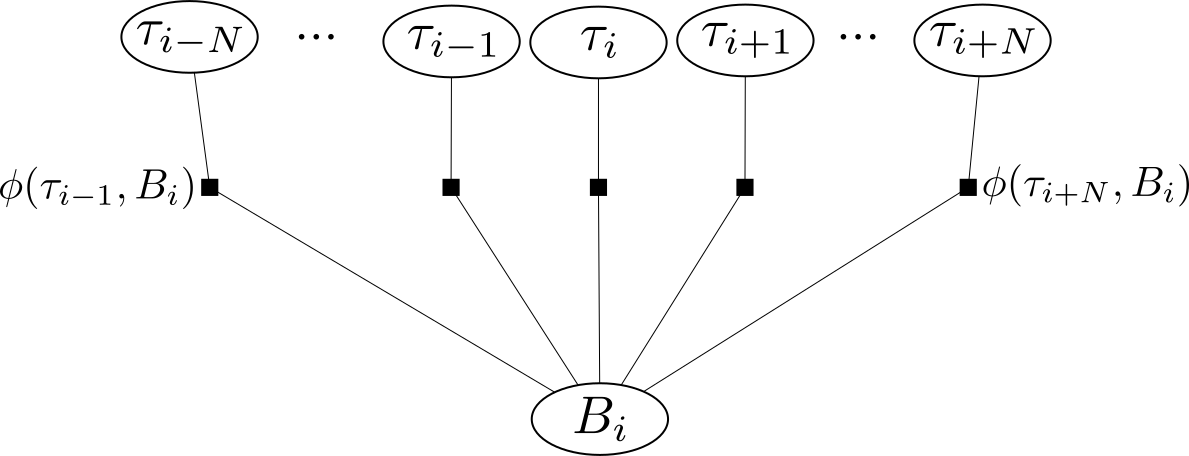
\includegraphics[scale=0.35]{burst-model-factor-graph.pdf}
\caption{The factor graph representation of the Bayesian burst-finding
algorithm. Here, $\tau$ denotes a photon inter-arrival time. $B_i$ is
a boolean variable indicating whether photon $i$ is due to a
burst. Note that the nodes $\tau_{i-N+1} ... \tau_{i-2}$ and
$\tau_{i+2} ... \tau_{i+N-1}$ have been omitted for consiseness.}
\end{figure}

\begin{equation}
  \phi(\tau, B) = \left\{
    \begin{array}{l l}
      P(\tau \vert \lambda_\mathrm{Burst})  & B = \mathrm{Burst} \\
      P(\tau \vert \lambda_\mathrm{BG})     & B = \mathrm{BG} \\
    \end{array}
  \right.
\end{equation}

Here $P(\tau \vert \lambda)$ is given by the standard exponential
distribution, giving the distribution over interarrival times of a
homogenous Poisson process,
\[ P(\tau \vert \lambda) = \lambda e^{-\tau \lambda} \]
We should acknowledge that for diffusing molecules the Poisson assumption
holds quite poorly. Thankfully, when $\lbg \ll \lburst$ the difference
is clear enough that the model continues to be quite effective.

\appendix
\section{References}
\bibliographystyle{plain}
\bibliography{burst-model.bib}

\end{document}
